\section{Asset Allocation with Transaction Costs}

\begin{frame}{Problem Formulation}
	\onslide<1->{
	\begin{block}{Investor's Goal}
		How to dynamically invest the available capital in a portfolio of different assets in order to maximize the expected total return or another relevant performance measure.
	\end{block}
	}
	

	\onslide<2->{
	\textbf{Rewards}: portfolio log-return with transaction costs
		\begin{equation*}
		 R_{t+1} = \log \left\{ 1 + \sum^{I}_{i=0} \left[ a_t^i X_{t+1}^i - \delta_i
		 			 	\left| a_t^i - \tilde{a}_t^i \right| - \delta_s {(a_t^i)}^- \right] -
		 			 	\delta_f \mathbf{1}_{{a}_t \neq \tilde{{a}}_{t-1}}\right\}
		 \end{equation*}
	}

	\onslide<3->{
	\textbf{Actions}: Portfolio weights
		\begin{equation*}
			\{a_t^i\}_{i=0}^I \;\;\; \text{s.t.}\;\;\; \sum^{I}_{i=0} a_t^i = 1 \;\;\;\;\; \forall t \in \{0, 1, 2, \ldots\}
		\end{equation*}
	}

	\onslide<4->{
	\textbf{States}: assets past returns and current allocation
		\begin{equation*}
			S_t = \{X, X_t, X_{t-1}, \ldots, X_{t-P}, \tilde{a}_t\}
		\end{equation*}
	}
\end{frame}

\begin{frame}[c]{Synthetic Asset: Convergence}
\begin{figure}[t!]
	\centering
	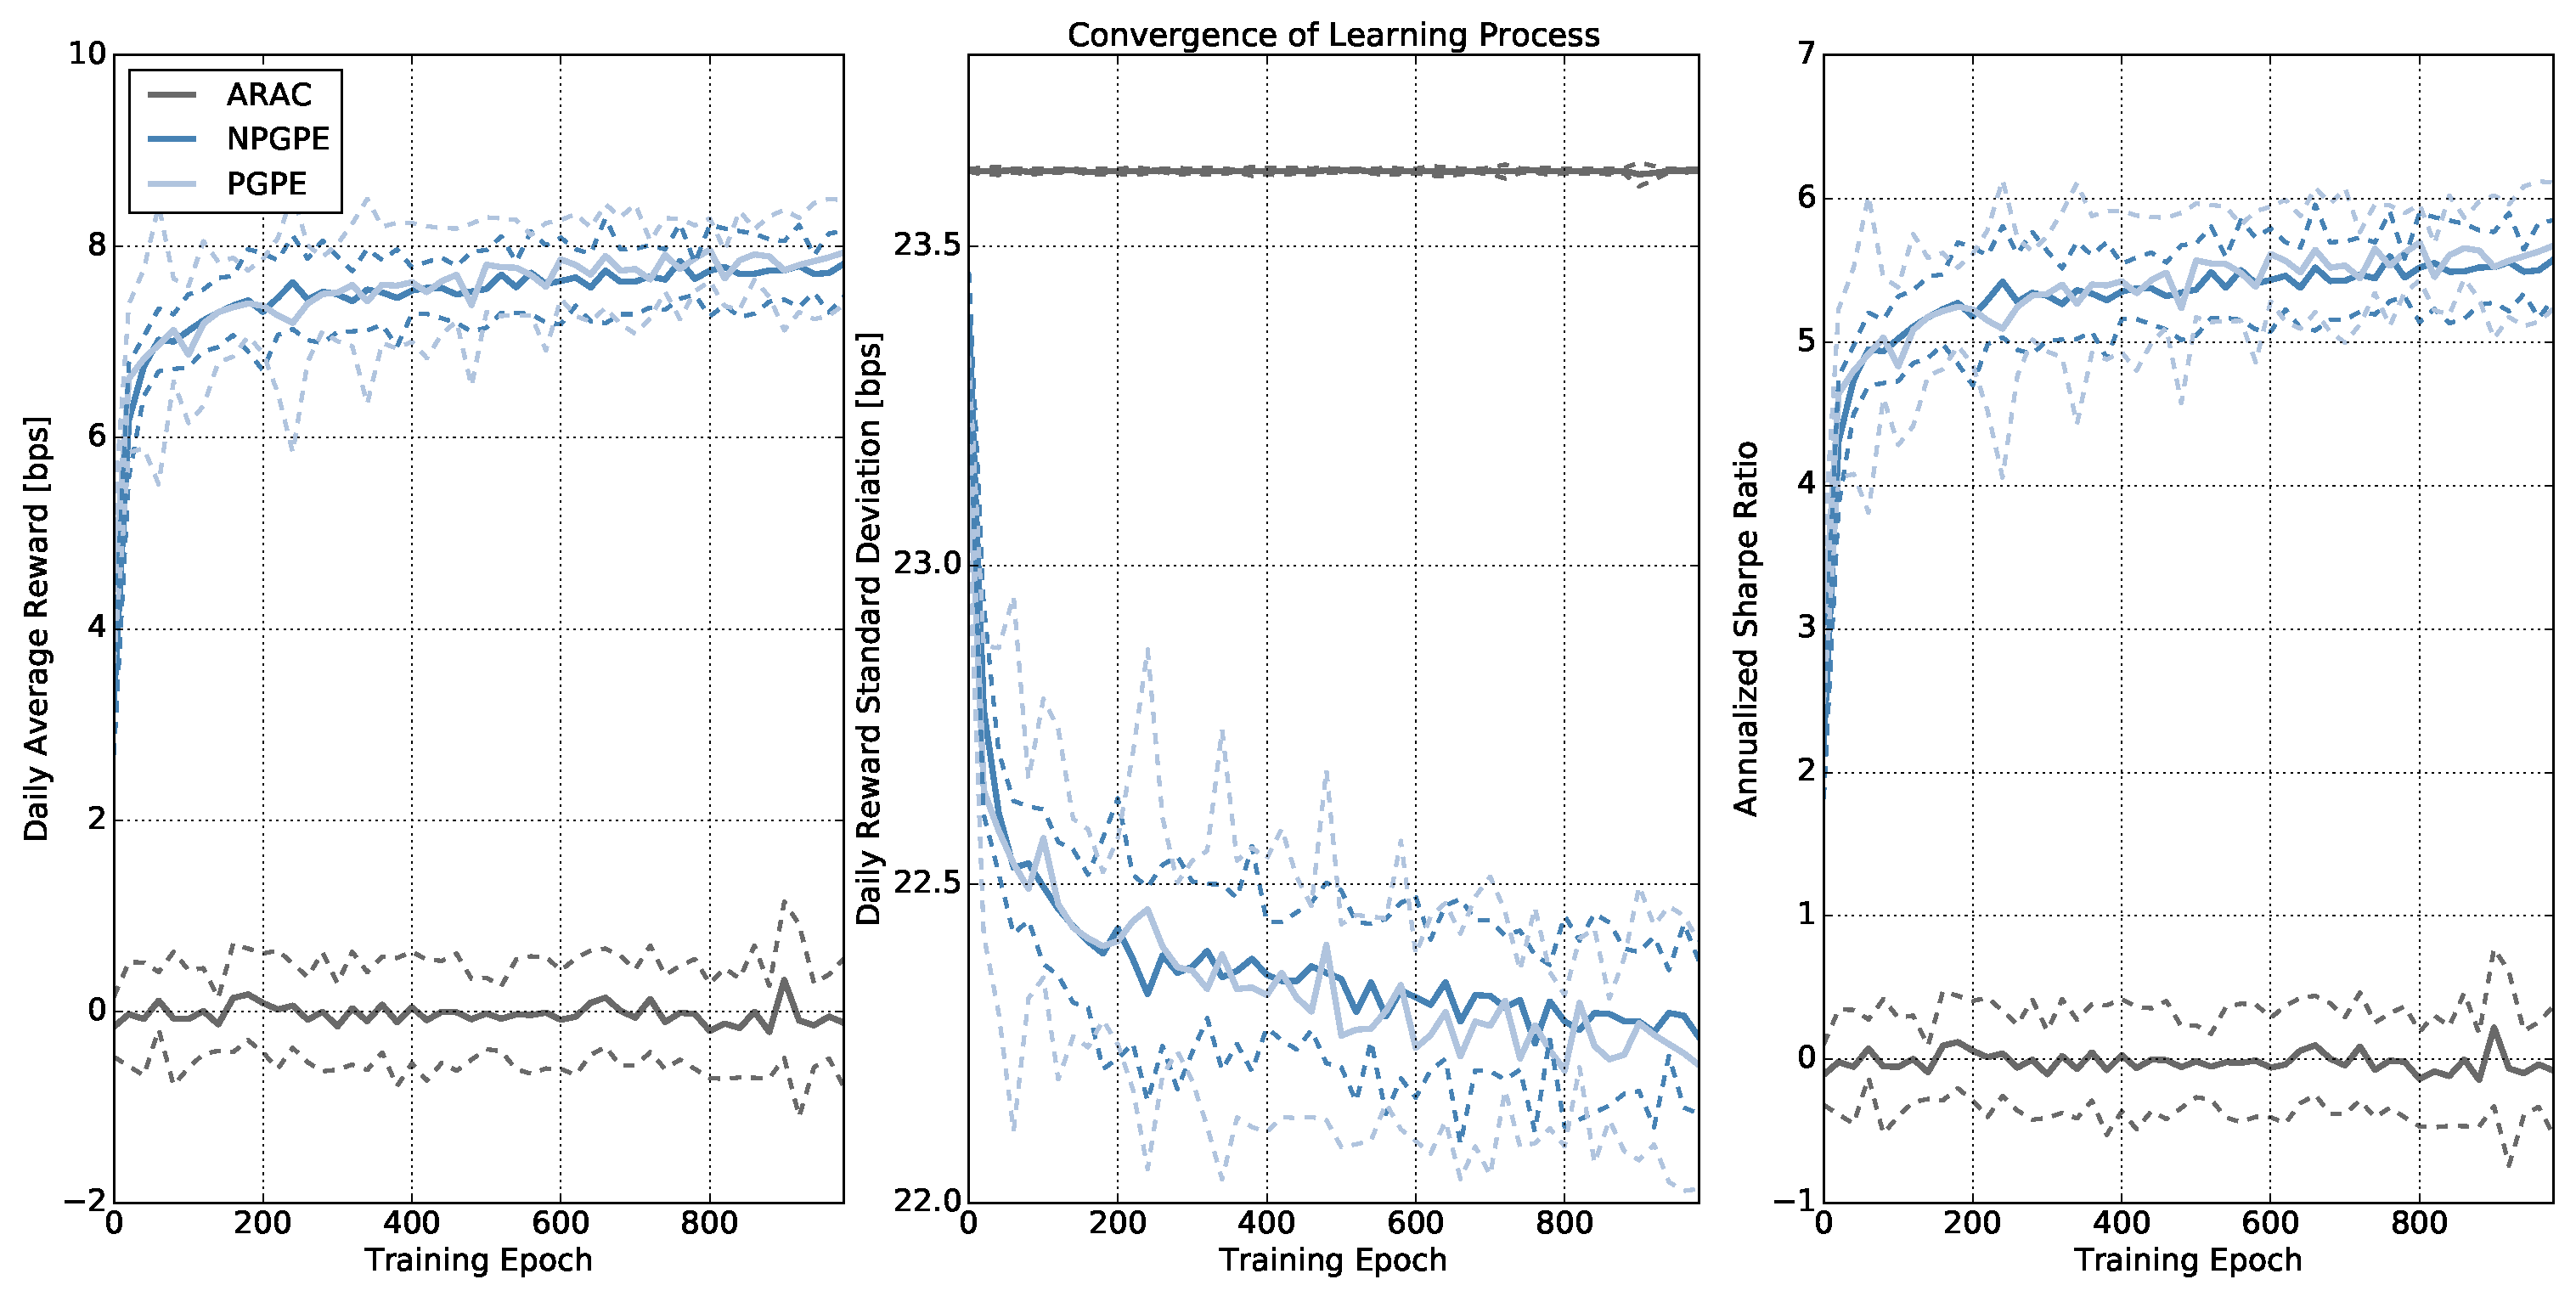
\includegraphics[height=5cm,width=0.8\textwidth]{Images/6_0_single_synthetic_neutral_convergence}
\end{figure}
\end{frame}


\begin{frame}[c]{Synthetic Asset: Backtest Performance}
\begin{figure}[t]
	\centering
	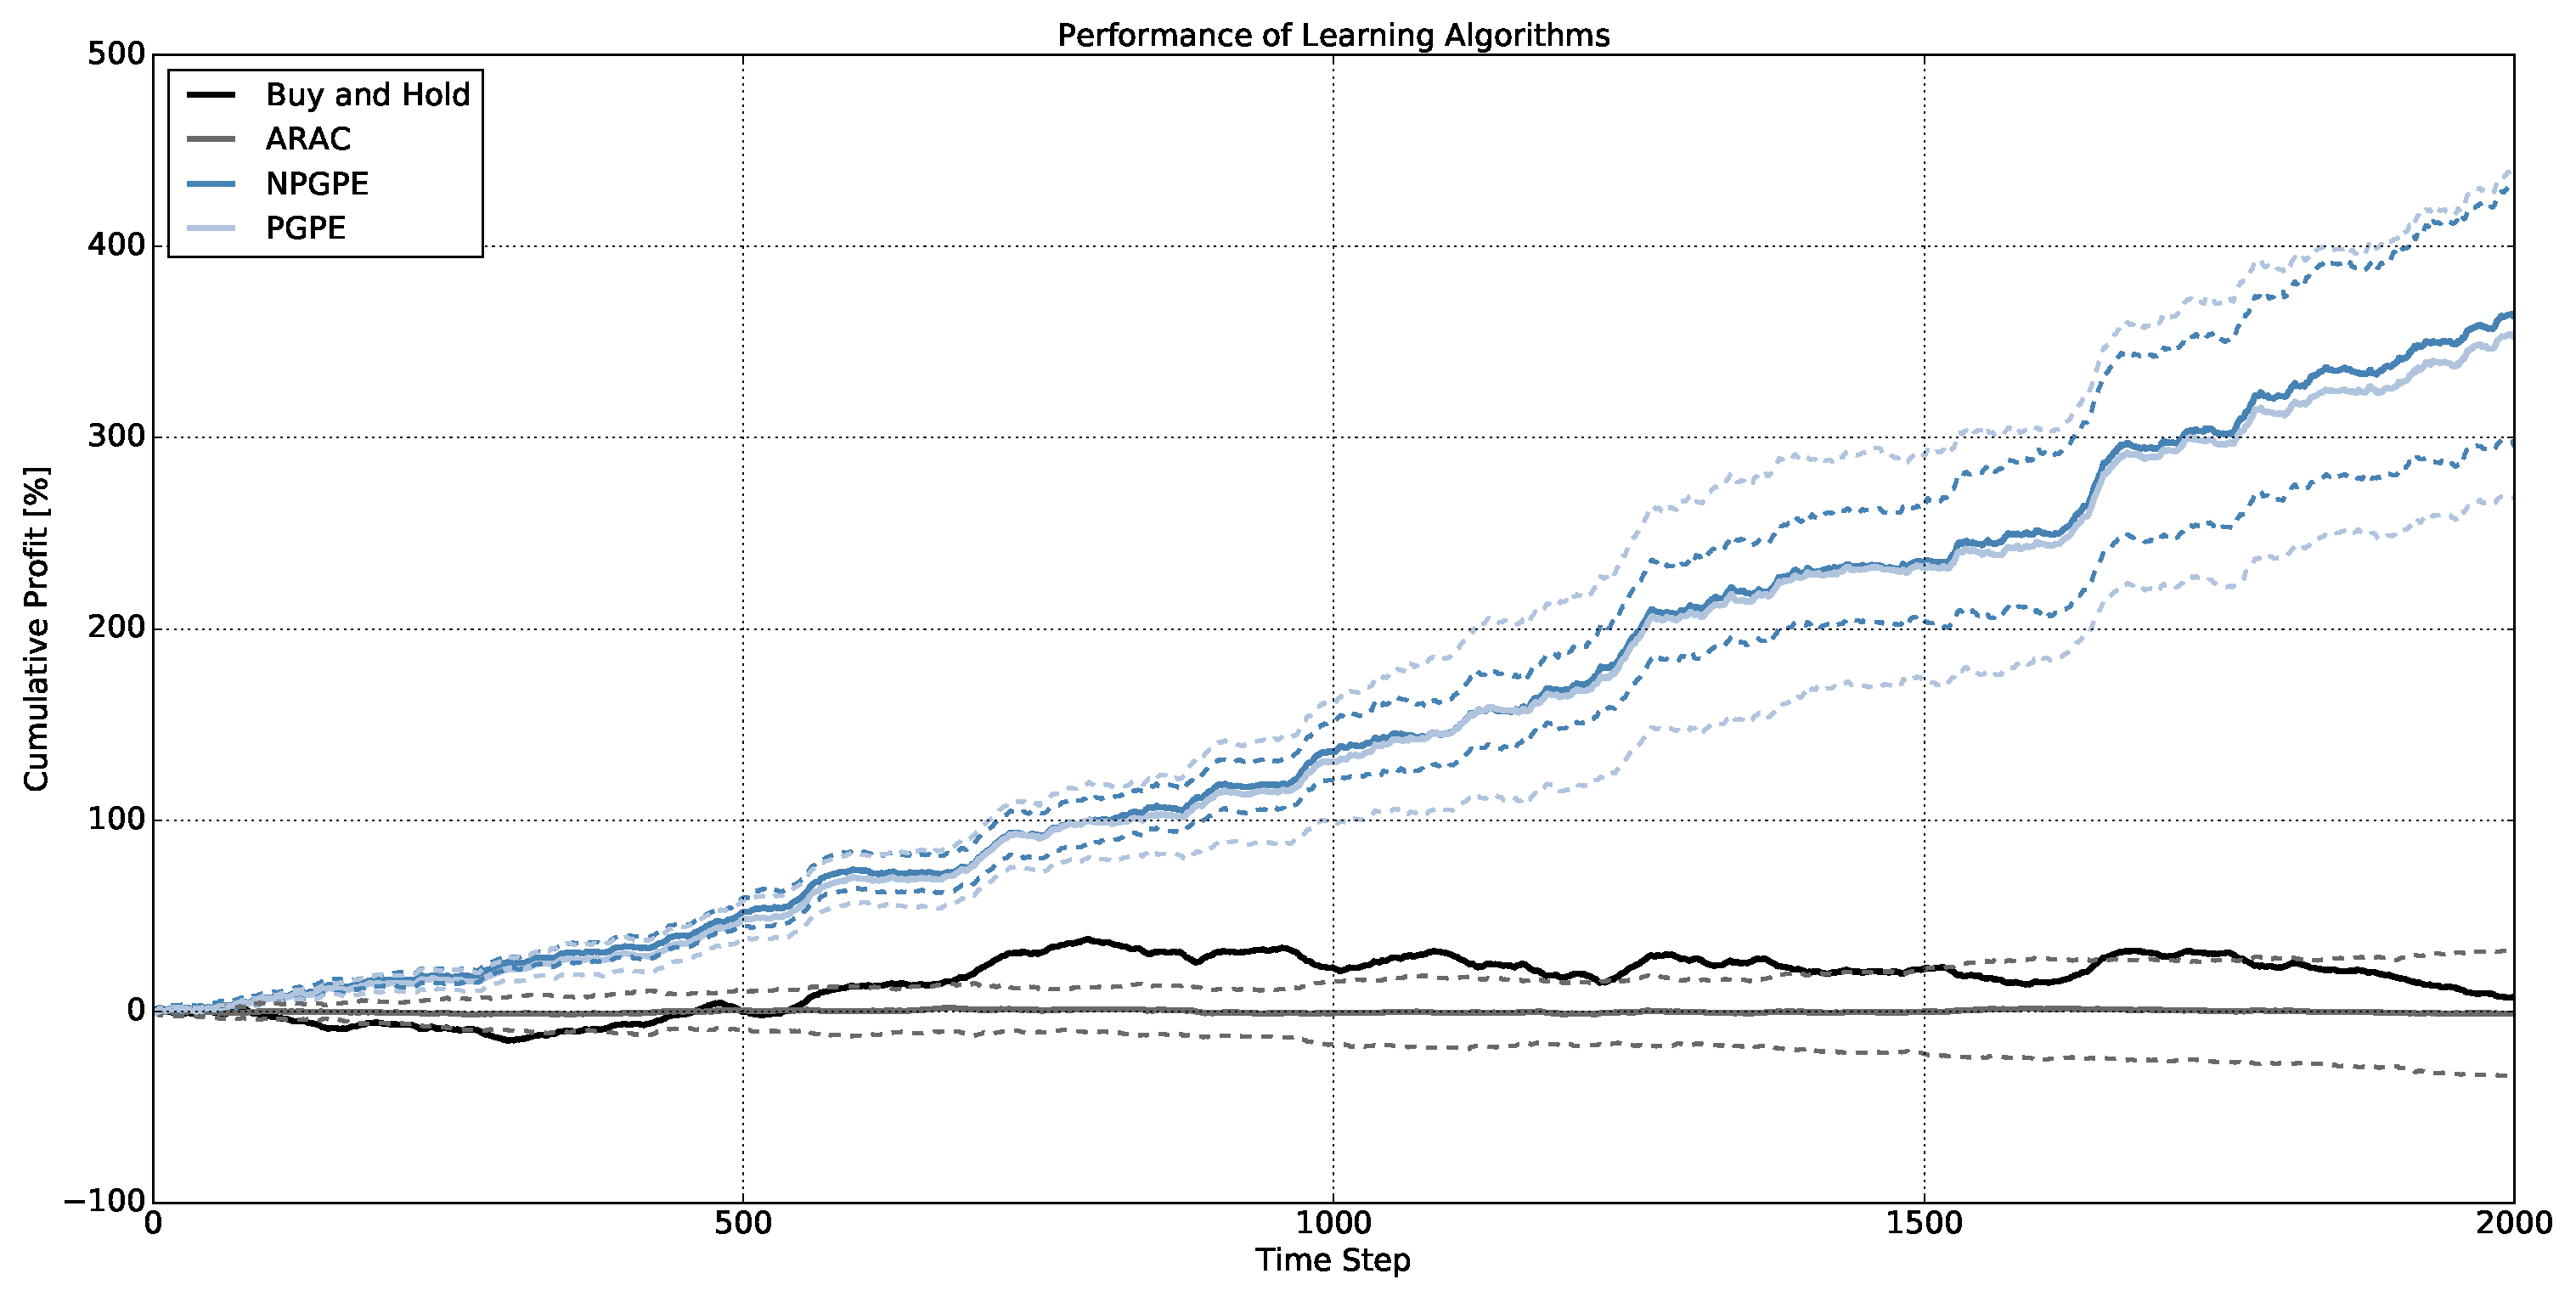
\includegraphics[height=6cm,width=0.8\textwidth]{Images/6_1_single_synthetic_neutral_performance}
\end{figure}
\end{frame}

\begin{frame}[c]{Synthetic Asset: Impact of Transaction Costs}
\begin{figure}[t!]
	\centering
	\includegraphics[height=3cm,width=0.8\textwidth]{Images/6_2_impact_transaction_costs}
\end{figure}
\begin{figure}[t!]
	\centering
	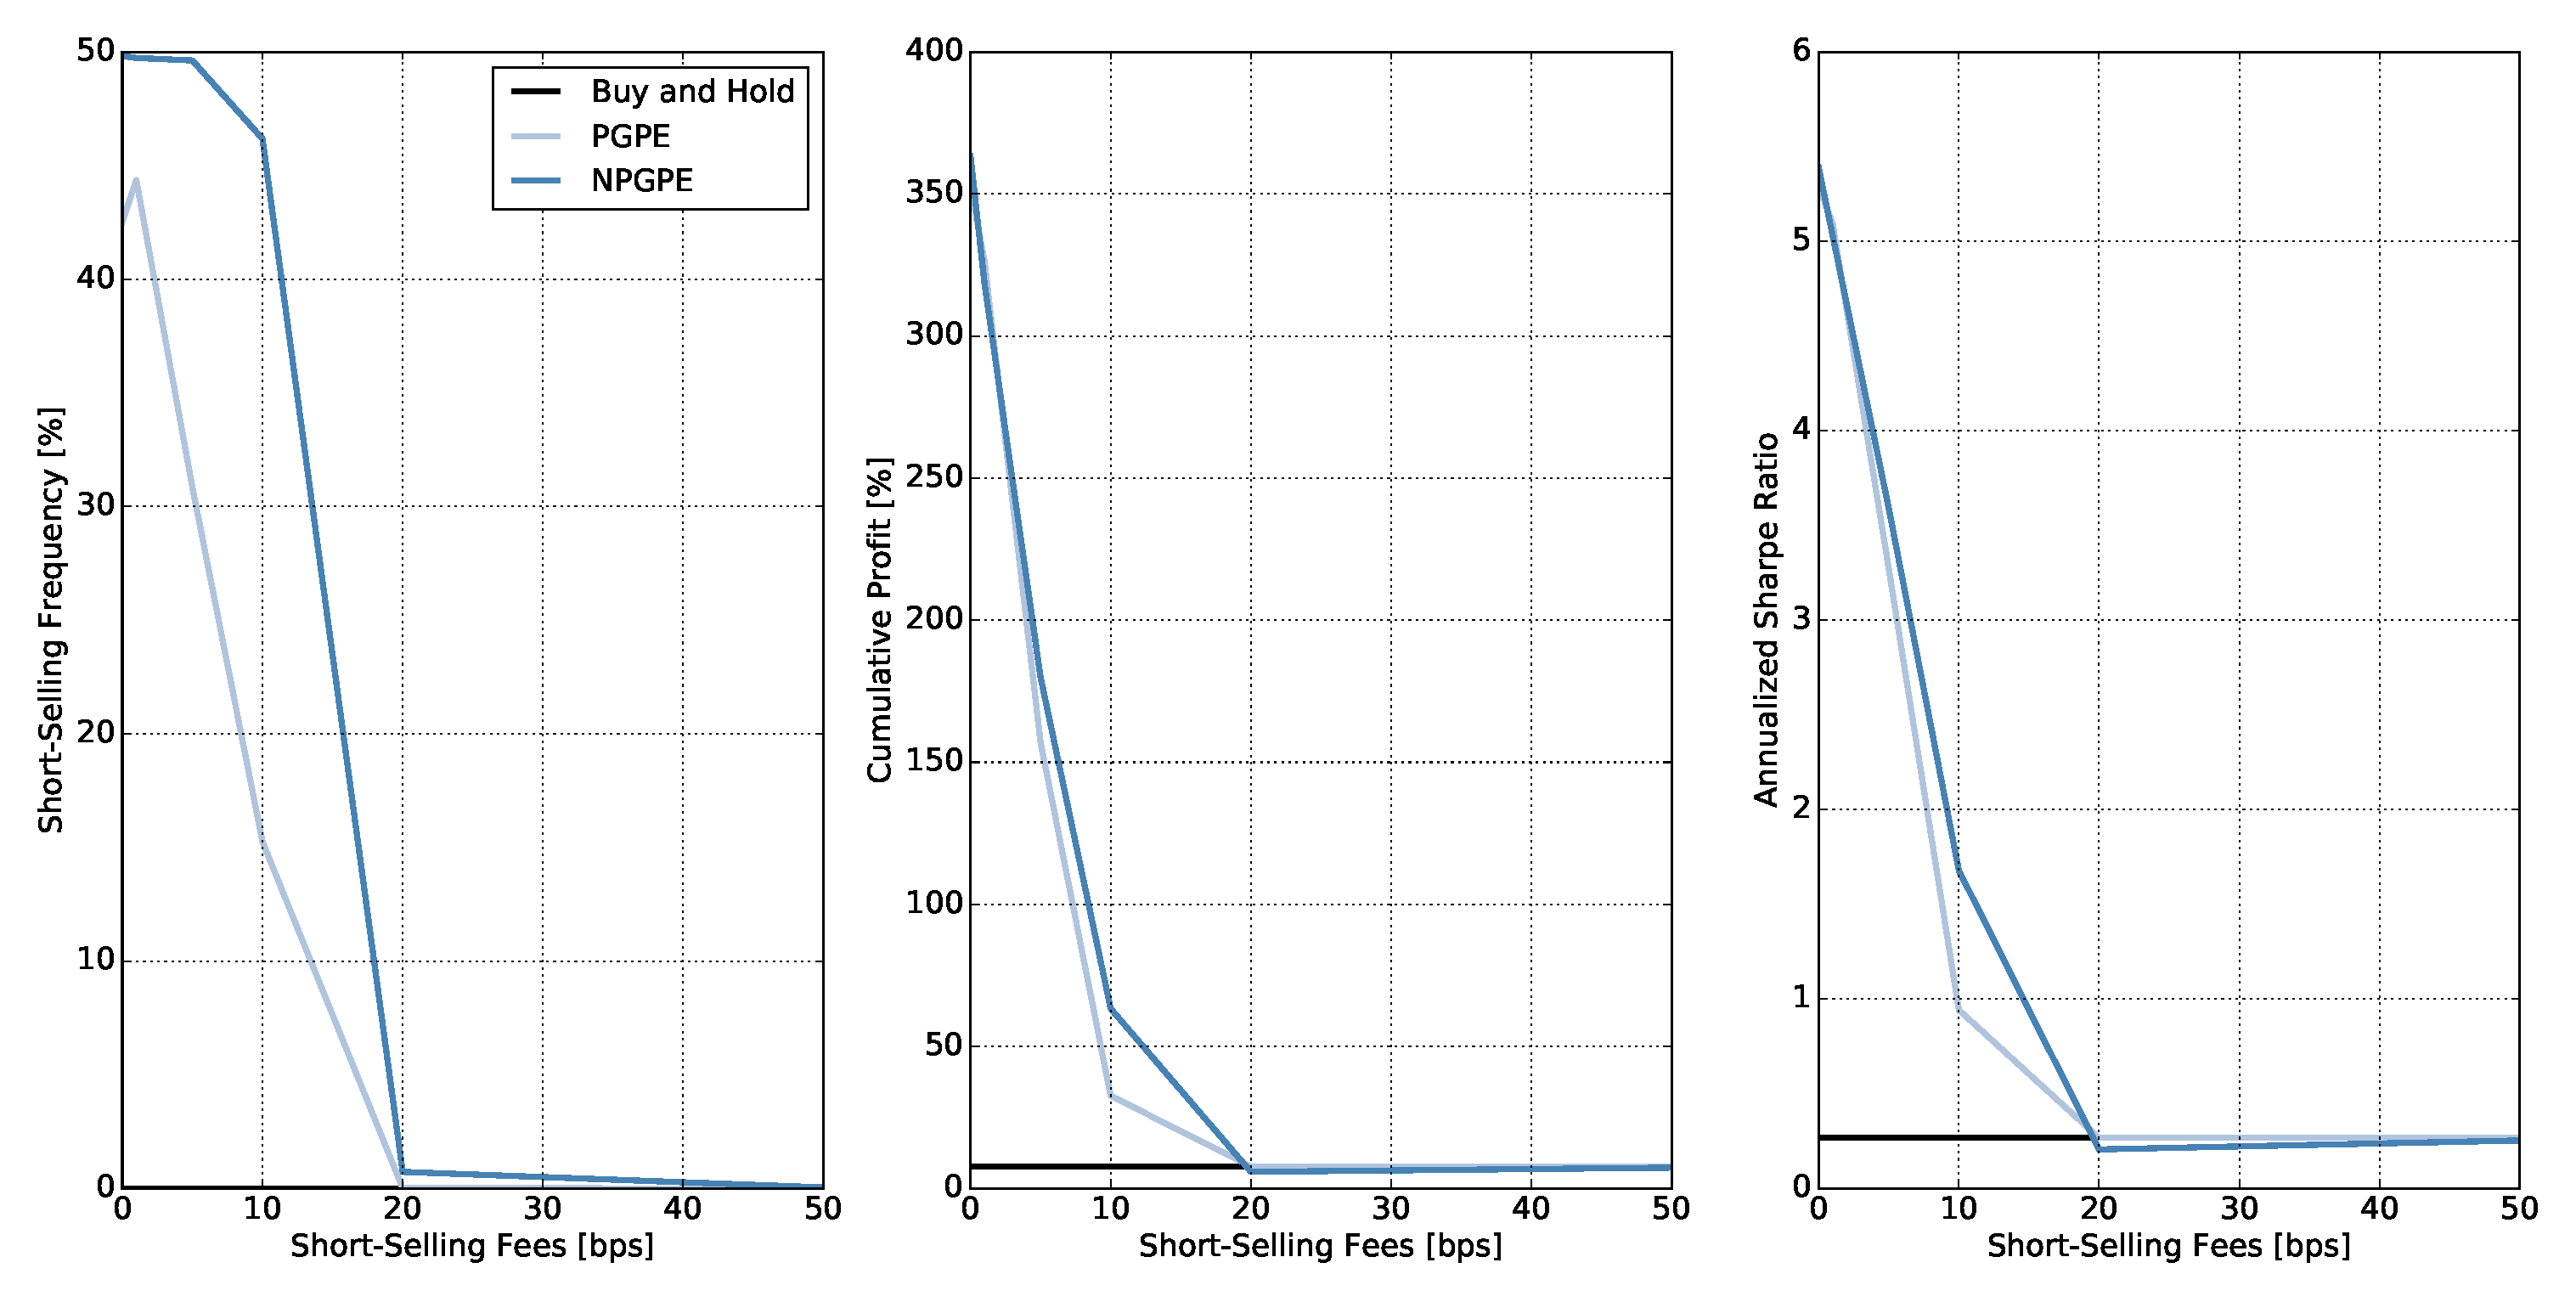
\includegraphics[height=3cm,width=0.8\textwidth]{Images/6_3_impact_short_selling_fees}
\end{figure}
\end{frame}

\begin{frame}{The Challenge of Historical Data}

\end{frame}

